\documentclass{article}

\usepackage{geometry}
\usepackage{amsthm}
\usepackage{amsmath}
\usepackage{graphicx}
\usepackage{amssymb}
\usepackage{latexsym}
\usepackage{bm}
\usepackage{xcolor}
\usepackage{mathtools}
\usepackage[toc,page]{appendix}
\usepackage{titlesec}
\usepackage{bbm}
\usepackage{caption}
\usepackage{hyperref}
\usepackage{float}
\usepackage{subcaption}

\newtheorem{theorem}{Theorem}[section]
\newtheorem{problem}[theorem]{Problem}
\newtheorem{lemma}[theorem]{Lemma}
\newtheorem{example}[theorem]{Example}
\newtheorem{definition}[theorem]{Definition}
\newtheorem{fact}[theorem]{Fact}
\newtheorem{post}[theorem]{Postulate}

\newcommand{\plot}[1]{
\begin{center}
\textcolor{blue}{\textbf{#1}}
\end{center}
}

\begin{document}
\title{The final report}
\maketitle
\section{State of project as of October 2023}

Since March till September 2023 I have been developing my implementation of the SPIDER technique, which is a method of measuring ultra-short laser pulses. Both the theory and the results I achieved I described in a detail way in my bachelor thesis ``To measure a laser pulse billion times shorter than a blink of an eye - the SPIDER technique''. This method is based on a idea of mixing two copies of a single pulse, while one of them is both delayed in time and spectrally shifted. The result is then measured by some kind of spectrometer, which shows the interference fringes containing information about the spectral phase of the initial pulse. The spectrum shown by the spectrometer is given by the equation:
\begin{multline}
I_{OSA}(\omega) = \left|\sqrt{I(\omega)}e^{i(\varphi(\omega)-\omega\tau))}+\sqrt{I(\omega-\Omega)}e^{i\varphi(\omega-\Omega)}\right|^2 = I(\omega) + I(\omega-\Omega) +\\
\sqrt{I(\omega)I(\omega-\Omega)}\left(e^{i(\varphi(\omega)+\omega\tau-\varphi(\omega-\Omega))}+e^{i(-\varphi(\omega)-\omega\tau+\varphi(\omega-\Omega))}\right) =\\
= \underbrace{I(\omega) + I(\omega-\Omega)}_\text{DC} + \underbrace{2\sqrt{I(\omega)I(\omega-\Omega)}\cos(\omega\tau + \textcolor{red}{\varphi(\omega) - \varphi(\omega-\Omega)})}_\text{AC}.
\end{multline}

The resulting spectrum has the slowly-varying DC component and fast-varying AC component, which posseses the information about \emph{spectral phase difference} marked in red. Using the Takeda algorithm one can extract that quantity and later estimate the spectral phase. Knowing both the spectral phase and the spectral intensity we can reconstruct the time-dependent electric field.

The setup that I utilized to perform my measurements is shown in fig. \ref{setup}.

\begin{figure}[h]
\caption{Final setup scheme}
\centering
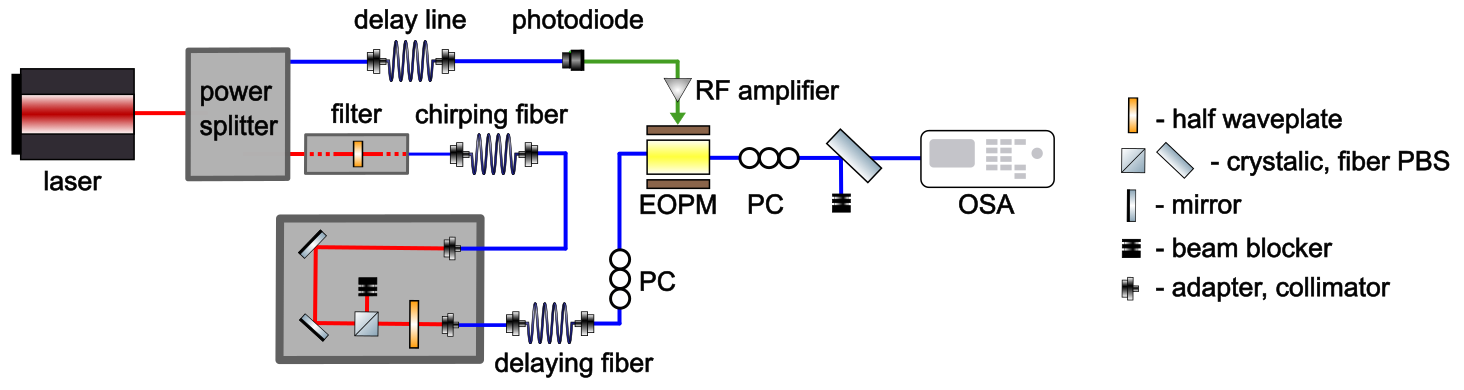
\includegraphics[scale = 0.6]{setup}
\label{setup}
\end{figure}

Although, as of the September my results were not complete, they were quite promising. I was testing my implementation of SPIDER with the chirp phase, which was introduced by propagation through an optical fiber and whose model is well-known. The reconstructed spectral phase shown in fig. \ref{final phase} matches quite good with the model.

\begin{figure}[h]
\caption{Reconstructed spectral phase vs. chirp model}
\subcaptionbox*{a) Chirp by PM fiber 80+20+4m}[.5\linewidth]{%
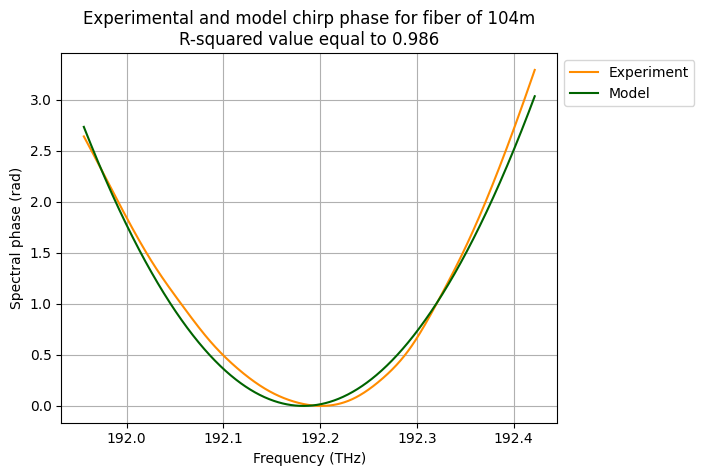
\includegraphics[width=\linewidth]{final_20}%
}%
\hfill
\subcaptionbox*{b) Chirp by PM fiber 80+40+4m}[.5\linewidth]{%
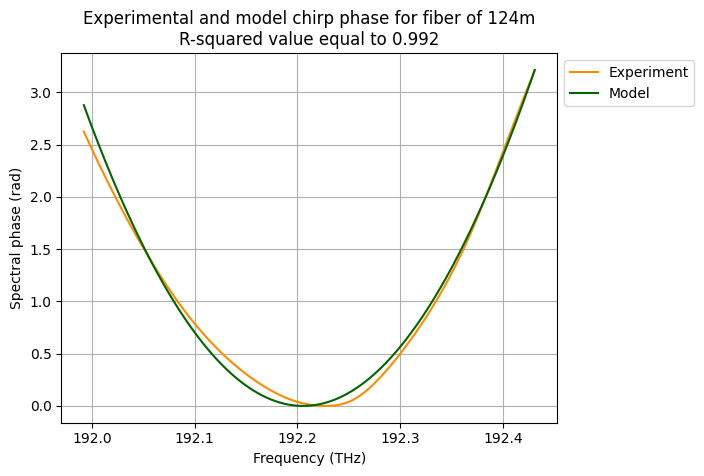
\includegraphics[width=\linewidth]{final_40}%
}
\label{final phase}
\end{figure}

\section{Stability}

Before defending my bachelor thesis I managed to perform only two measurements, which seemed to be done in a correct way. The next step was therefore testing the system stability, i. e. repeating the measurements in the identical (or at least comparable) conditions and checking, if the results are the same as previously. \textbf{They were not.}

The model was all the time the chirp phase, which should result in a parabolic shape of the spectral phase. And, although the obtained curves were parabolic indeed, they were scaled, i. e. the coefficient before the parabola did differ from the one predicted by the model. Moreover, the scaling factor wasn't constant throughout the subsequent experiments. As shown in my thesis the spectral phase model is equal to:
\begin{equation}
\varphi(\omega)=\frac{\lambda_0^2LD_\lambda}{4\pi c}(\omega-\omega_0)^2,
\end{equation}
where $\lambda_0$ denotes the central wavelength, $\omega_0$ denotes the central frequency, $L$ denotes the fiber length and the $D_\lambda$ denotes the dispersion parameter. The coefficient before the parabola may be therefore characterized by \emph{effective dispersion parameter} or \emph{effective fiber length}. I opted for using the second quantity, because if the laser pulse is already chirped after exiting the laser cavity, this should result in a constant addition to the fiber length. I have found several reasons, which could explain the big variance of the effective fiber length:
\begin{enumerate}
\item \textbf{The initial laser pulse is already chirped.} This hipothesis must be still examined, but after some tries of fitting an effective fiber length $L \to L+L_0$ I did not manage to find a constant value of $L_0$, which would match with experiments' outcome.

\item \textbf{The value of the dispersion parameter is wrong}. The value of dispersion parameter for fused silica given by \emph{RP photonics} is equal 20 ps/(nm$\cdot$km). Dr Michał Karpiński told me that it is equal to 17 ps/(nm$\cdot$km). The theoretical model derived in my thesis suggests that this is equal to 15 ps/(nm$\cdot$km). This divergence \textbf{must} be explained. Possibly the best way of finding the exact value of the dispersion parameter is measuring it in a separate experment. However, even the incorrect value of the dispersion parameter used to predict experiment's outcome, does not fully explain the huge variance of the results.

\item \textbf{Chirping in the EOP modulator}. This can be caused be two independent factors: a \emph{regular} chirping in the lithium niobate or not fully linear current going through the modulator. However, I must perform some simulations, which could verify, if indeed a slight deviation from linear current (something like $o(t^2)$ or $o(t^3)$) could cause an effect similar to chirping. \\

\hspace*{1cm}
\begin{minipage}{.8\textwidth}
\textbf{Digression:} Anyway, it is crucial, to make sure that the shear applied by the EOPM is fully linear and homogeneous. This can be performed by connecting a Python software to OSA and comparing the spectrum before and after a spectral shear. The \emph{good} shear would be such, that after \emph{deshearing} (for example, shifting one spectrum in postprocessing so that both spectra have the same central wavelength) the mean squared error between both spectra is minimized. However, another approach is also available. The project that we are pursuing together with Jerzy Sz. and Michał Ch. is about finding a phase suitable for performing any transformation between two spectra. Employing the model trained within this project, I could find the spectral phase directly and thereby ensure that it is linear. This would also make a wonderful papers title: \emph{AI-enhanced SPIDER}. Of course, this would be another senseless utilization of ML methods: since I know that the temporal phase is close to an linear one, I could use the classical methods to fit the coefficients before $\omega^2$, $\omega^3$, etc.
\end{minipage}

\item \textbf{The inexact shear measurement} As I pointed out already in my thesis the choice of method for measuring the shear is of highest importance (overestimating the shear $\alpha$ times results in the spectral phase scaled by the factor of $1/\alpha$. And the problem is not measuring the sheared and not-sheared spectrum, but simply computing numerically the shift between them. If the spectra did not exhibit any noise, then all the methods should give the very same answer. Unfortunately, it is just the opposite. 
\end{enumerate}

I identified the 4th point from the above list as the responsible for greatest part of the spectral phase variance. However, it needs to be stressed that \textbf{other problems can not be neglected neither}. Obviously, it is possible that there exists also another important factor, which I was unable to notice.

I have developed 4 techniques of measuring the shear: \textbf{fit} - finding such a spectral shift that minimizes the MSE between both spectra in postprocessing; \textbf{com} - estimating the shear as the difference between centers of mass (central frequencies) of both spectra; \textbf{rect} - fitting rectangles to the spectra and computing the shear as the mean shift of the rectangles' sides;  \textbf{slope} - for both spectra compute the lowest frequency, where the intensity is higher that 0.1 of the maximal one. Repeat this for 100 points with the thresholds from 0.1 to 0.3 for both left and the right side. The shear is now estimated as the mean of the shifts of these threshold frequencies. 

Note, that when the value of the shear is of the same order as the frequency spacing, then some kind of interpolation should be performed (otherwise the values of the shear might turn out to be discrete). This is crucial in the case of the \textbf{fit} method and may improve the accuracy of the \textbf{rect} and \textbf{slope} methods.

I performed several new measurements and also utilized the old ones to verify, which of the above methods is the most accurate. For each reconstructed parabolic spectral phase I found an effective fiber length that would result in a phase most similar to the experimental one. Obiously, the goal is to obtain \emph{effective fiber length} $\simeq$ \emph{fiber length}. The results are shown in fig. \ref{historic measurements}.

\begin{figure}[h!]

\caption{Effective vs. real fiber length - comparison of methods measuring shear}
\subcaptionbox*{a) Center of mass}[.48\linewidth]{%
\includegraphics[width=\linewidth]{Reconstructions_effects_com}%
}%
\hfill
\subcaptionbox*{b) Minimizing MSE}[.48\linewidth]{%
\includegraphics[width=\linewidth]{Reconstructions_effects_fit}%
}

\vfill

\subcaptionbox*{c) Fitting a rectangle}[.48\linewidth]{%
\includegraphics[width=\linewidth]{Reconstructions_effects_rect}%
}%
\hfill
\subcaptionbox*{d) Slope shift}[.48\linewidth]{%
\includegraphics[width=\linewidth]{Reconstructions_effects_slope}%
}
\label{historic measurements}
\end{figure}

It is quite clear that the \textbf{slope} method is the best. However, looking at the curve constructed of the measurements data (I mean, imagine a line going through the colorful points in the d) plot), one could say that the laser pulse is initially negatively chirped and at the same time the dispersion parameter is even greater than 20 ps/(nm$\cdot$km).  Could it be so? There's only one way of checking this - more measurements.

To verify the above hipothesis (and also check, if the \textbf{slope} method is, indeed, the best one) I performed two series of measurements. In one experiment I used the total length of 84 m of fiber introducing the parabolic spectral phase and in the second one I used 124 m of the same fiber. Each experiment constisted of several measurements for different values of shear. The first goal of the experiment was to find the best shear measuring method. For such a method the effective fiber length should be constant, no matter what shear was applied. I did also monitor the relationship between the value of the shear and the value of power given on the photodiode. Ideally, it should be linear (at least for the low powers). Finally, since the measurements were performed for two different lengths of fiber, I utilized them to estimate the value of the dispersion parameter \textbf{and} the value of the chirp phase, which is independent of the fiber length (this includes the intitial chirp) (this quantity is characterized by an additional, constant fiber length $L\to L+L_0$). The measurements of effective fiber length for the setup characterized by the fiber length 84 m are shown in fig. \ref{fiber_84}. I'd like to stress, that - contrary to the resuls depicted on fig. \ref{historic measurements} - the following were performed in a one day session.
 
\begin{figure}[H]

\caption{Effective vs. real fiber length - 84 m}
\subcaptionbox*{a) Center of mass}[.48\linewidth]{%
\includegraphics[width=\linewidth]{best_fit_fiber_com_1}%
}%
\hfill
\subcaptionbox*{b) Minimizing MSE}[.48\linewidth]{%
\includegraphics[width=\linewidth]{best_fit_fiber_fit_1}%
}

\vfill

\subcaptionbox*{c) Fitting a rectangle}[.48\linewidth]{%
\includegraphics[width=\linewidth]{best_fit_fiber_rect_1}%
}%
\hfill
\subcaptionbox*{d) Slope shift}[.48\linewidth]{%
\includegraphics[width=\linewidth]{best_fit_fiber_slope_1}%
}
\label{fiber_84}
\end{figure}

In the fig. \ref{photodiode_84} the relation between power on photodiode and the value of the shear is shown.

\begin{figure}[H]

\caption{Shear vs. photodiode power - 84 m}
\subcaptionbox*{a) Center of mass}[.48\linewidth]{%
\includegraphics[width=\linewidth]{PD_vs_shear_com_1}%
}%
\hfill
\subcaptionbox*{b) Minimizing MSE}[.48\linewidth]{%
\includegraphics[width=\linewidth]{PD_vs_shear_fit_1}%
}

\vfill

\subcaptionbox*{c) Fitting a rectangle}[.48\linewidth]{%
\includegraphics[width=\linewidth]{PD_vs_shear_rect_1}%
}%
\hfill
\subcaptionbox*{d) Slope shift}[.48\linewidth]{%
\includegraphics[width=\linewidth]{PD_vs_shear_slope_1}%
}
\label{photodiode_84}
\end{figure}

The analogous measurements performed on a setup with the 124 m long fiber are shown in the figures \ref{fiber_124} and \ref{photodiode_124}.
 
\begin{figure}[H]

\caption{Effective vs. real fiber length - 1244 m}
\subcaptionbox*{a) Center of mass}[.48\linewidth]{%
\includegraphics[width=\linewidth]{best_fit_fiber_com_2}%
}%
\hfill
\subcaptionbox*{b) Minimizing MSE}[.48\linewidth]{%
\includegraphics[width=\linewidth]{best_fit_fiber_fit_2}%
}

\vfill

\subcaptionbox*{c) Fitting a rectangle}[.48\linewidth]{%
\includegraphics[width=\linewidth]{best_fit_fiber_rect_2}%
}%
\hfill
\subcaptionbox*{d) Slope shift}[.48\linewidth]{%
\includegraphics[width=\linewidth]{best_fit_fiber_slope_2}%
}
\label{fiber_124}
\end{figure}
 
\begin{figure}[H]

\caption{Shear vs. photodiode power - 124 m}
\subcaptionbox*{a) Center of mass}[.48\linewidth]{%
\includegraphics[width=\linewidth]{PD_vs_shear_com_2}%
}%
\hfill
\subcaptionbox*{b) Minimizing MSE}[.48\linewidth]{%
\includegraphics[width=\linewidth]{PD_vs_shear_fit_2}%
}

\vfill

\subcaptionbox*{c) Fitting a rectangle}[.48\linewidth]{%
\includegraphics[width=\linewidth]{PD_vs_shear_rect_2}%
}%
\hfill
\subcaptionbox*{d) Slope shift}[.48\linewidth]{%
\includegraphics[width=\linewidth]{PD_vs_shear_slope_2}%
}
\label{photodiode_124}
\end{figure}
 
The results of measurements (especially the figures \ref{fiber_84} and \ref{fiber_124} suggest that definetely two best methods of measuring the shear are the \textbf{slope} and the \textbf{rect} method. However, as I found out later, the \textbf{rect} method works good only under the condition that the spectrum, well... is rectangular, i. e. has a wide support with quite constant intensity and steep slopes. When this method is applied, for example to the first hermite-gaussian mode of intensity, the results are much worse. Summing things up, I chose the \textbf{slope} method and have been using it till now.

The good news is that the results obtained with this method are indeed constant within wide range of shears and the relationship between the power and the shear is linear. We can try to estimate the values of the dispersion parameter and the \emph{offset} chirp phase characterized by an additional (and artificial) fiber length $L_0$. We do it by comparing the tabulated value of the dispersion parameter and effective fiber length on the one side and the actual fiber length with offset, together with predicted dispersion parameter on the other:

\begin{equation}
L_{eff}\cdot D_{\lambda tab}=(L_{actual}+L_0)\cdot D_{\lambda pred}
\end{equation}

Now we simply must solve a system of equations:

\begin{equation}
\left\{\begin{array}{ll}
88.5\cdot 20=(84+L_0)\cdot D_{\lambda pred}\\
112.2\cdot 20=(124+L_0)\cdot D_{\lambda pred}
\end{array}\right.
\end{equation}

\begin{equation}
\left\{\begin{array}{ll}
D_{\lambda pred} = 11.85\textrm{ ps}/(\textrm{nm}\cdot\textrm{km})\\
L_0 = 65.4\textrm{ m}
\end{array}\right.
\label{disp_exp}
\end{equation}
 
Well, the results obtained above are not completely out of the world, but they aren't very plausible at the same time. The value of the dispersion parameter is much lower than expected, while value of an additional chirp is rather to high. Since the results within a single serie of measurements were rather consistent, one could suspect a systematic error, i. e. an error that biased the entire serie of measurements. This \textbf{could} be caused by a not fully linear shear applied by the EOPM - only the intensity of the current steering the modulator was modifed for subsequent measurements, the shape of the current (i. e. relative delay applied by delay line) remained constant and it could be just this shape that had been a problem.

Personally, I do not think of the results \ref{disp_exp} as convincing. I believe that it would be best to measure the dispersion parameter in a separate measurement (as I have already mentioned before) and then try to estimate the additional chirp characterized by $L_0$.

But overall, the outcomes of this part of measurements are not that bad. When the \textbf{slope} method was applied, the results were consistent and stable within a single serie of measurements. What's more, the obtained spectral phases are almost perfectly parabolic - it's just the parabola's coefficient that was \textbf{slightly} scaled. If one wishes to obtain high resolution of SPIDER, obviously it is crucial to ensure that this coefficient is constant, but for now I decided to move on and to start measuring non-parabolic spectral phases.\\
\\

Four months after conducting the measurements shown above I came up with an idea, what might a problem. I still think that the reason for a systematic error - as described above - is the EOPM. But the reason might be  connected neither with nonlinear current nor with regular chirping in lithium niobate. In my bachelor thesis I assumed that the influence of the current on the refractive index of modulator's waveguide might be described effectively by the equation:

\begin{equation}
n(I)=n_0+n_1I,
\end{equation}

where the initial refractive index $n_0$ might be safely neglected, since it does not alter the shape of the pulse after leaving the modulator. And the value of $n_0$ should not change the shape of the spectral phase, indeed, but it may change the relative delay between polarization. If the \emph{mean} current overlapping with the optical pulse isn't zero, than the model should be:

\begin{equation}
n(I)=(n_0+\varepsilon)+n_1I,
\end{equation}

Maybe it is easier to explain this idea on a scheme (fig. \ref{mean_int}):

\begin{figure}[H]
\caption{Scheme depicting mean intensity problem}
\centering
\includegraphics[scale = 0.4]{mean_intensity}
\label{mean_int}
\end{figure}

Modification of refractive index by a constant adds a time delay, which results in an additional linear phase in spectral phase difference, which results in an additional quadratic phase in spectral phase. This might explain the repeatibilty within a single serie, but lack of it within two separate series (maybe the mean current was different first time than the second?).

I must perform exact calculations but I estimate that a relative delay of a femto- or even attosecond can result in a significant addition of a quadratic phase in the reconstructed spectral phase.

The funny thing is that the above hipothesis is \textbf{wrong} and I should rather try to explain why the above-described effect is \textbf{not} observed within the measurments. What am I talking about? To increase the shear, I must increase the current modulator and therefore I also increase the mean current. Hence, if this hipothesis had been correct, we should be able to see a linear dependance of the effective fiber length on the value of shear. This dependance is clearly not there, since the effective fiber length is almost constant for various shear values.

To match with the measurements the modification of the refractive index must be constant - maybe caused by optical rectification? I am not sure.

\pagebreak

\section{Non-parabolic phases}

With help of Filip Sośnicki I tested my implementation of SPIDER with some non-parabolic phases. The effects are shown in fig. \ref{non_parabolic}. The intensity spectrum is not shown (in the future I will make it show automatically), but only a spectral phase corresponding to non-zero intensity are plotted.

\begin{figure}[H]

\caption{Reconstruction of non-parabolic spectral phases}
\subcaptionbox*{a) 4th order polynomial}[.48\linewidth]{%
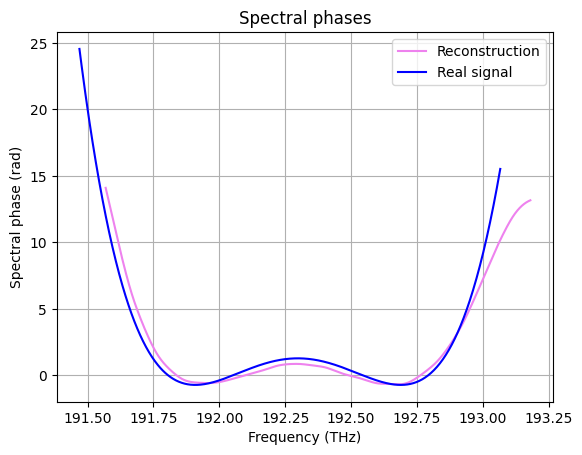
\includegraphics[width=\linewidth]{non_parabolic_1}%
}
\hfill
\subcaptionbox*{b) Slowly-varying sine}[.48\linewidth]{%
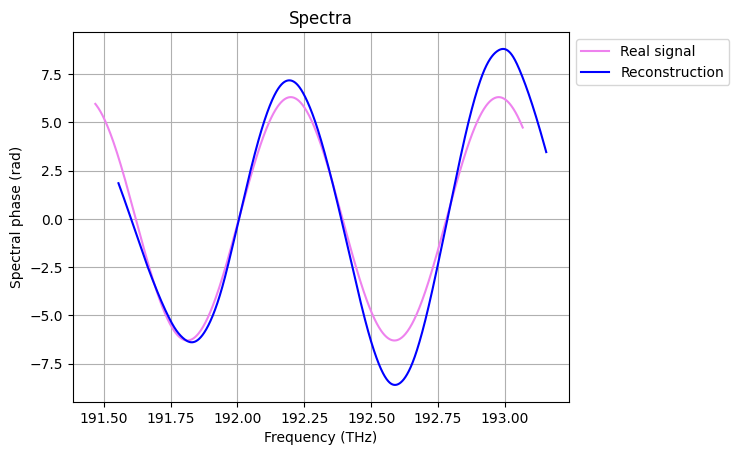
\includegraphics[width=\linewidth]{non_parabolic_2}%
}
\vfill
\subcaptionbox*{c) Rapidly-varying sine}[.48\linewidth]{%
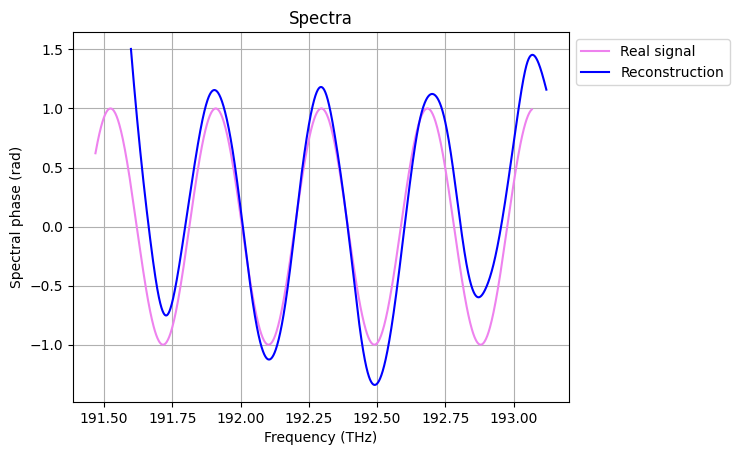
\includegraphics[width=\linewidth]{non_parabolic_3}%
}
\label{non_parabolic}
\end{figure}

The reconstruction is not perfect, but still it looks quite promising. The plot a) looks very nicely, but the phase on plot b) is scaled (once again problem with scaling!) on the right side of the plot. However, it is a good sign that the extrema of both curves on plot b) occur for the same frequencies. The curves on plot c) look better, but still we might observe a slight addition of a quadratic phase (problem we discussed before). Note, however, that the magnitude of spectral phase on plot c) is much smaller then on the two other plots, therefore it makes sense that the influence of unwanted parabolic phase is bigger.

\section{Testing resolution with hermite-gaussian modes}

Since the results shown in previous section looked promising, I was asked to check what is the lowest resolution, with which I would be able to measure the spectral phase. To make sense of the word \emph{resolution} I needed to work with rapidly changing phases. Simplest example of phase changing rapidly is an instant jump like in the \emph{signum} function. This way I started to deal with the hermite-gaussian modes.

\textbf{Digression:} The key factor controlling the resolution is the shear. The shear is the step with which I am sampling the spectral phase difference and thus the shear controlls the spacing of points of the measured spectral phase. One could think that the period of interference fringes is, as well, important and \emph{the more fringes, the better resolution}. However, I believe that it is an incorrect reasoning. The spectral phase, that we want, can be seen as a deviation from regular fringes resulting from time-mixing of two pulses alone. At the same time, the more fringes, the more rapidly they oscillate and the smaller is the influence of the constant spectral phase on the shape of the interferogram. Equivalently, we can think that the more fringes, the bigger is the fraction of temporal phase in the term $\omega\tau+\varphi(\omega) - \varphi(\omega-\Omega)$, that we isolate from the interferogram.

In the fig. \ref{hermite_1} I showed reconstruction effects of the spectral phase of hermite-gaussian modes. The phase should change its value by $\pi$ for these frequencies, where the electric field changes its sign (and the intensity \emph{bounces back} from the X-axis).

In the plot a) the spectral phase should be flat, but we can observe quite a lot of noise. Luckily, its amplitude is not big. \textbf{Digression:} Oscillations in the spectral phase with period of 65 GHz (not responsible for the entire noise) are cause by incorrectly connected PM fiber to the EOPM. Even with the polarization controller I am not able to fully compensate this effect.

The spectral phases on plots b) and c) look actually very nice. The phase changes rapidly in right places and its jumps are roughly equal to $\pi$. Moreover, I'd like to stress that the shear used in experiement (hence the resolution) is 11 GHz, which is quite a little. Obviously, this value is to be improved.

However, I believe that the quantity that we should watch more carefully is the spectral phase difference $\varphi(\omega)-\varphi(\omega-\Omega)$ and not the spectral phase $\varphi$ alone. It is the spectral phase difference, that we obtain directly from the measurment. Transition from spectral phase difference to spectral phase is a purely numerical process and is involved with loss of information, since we are sampling the first with the step equal to the shear. The spectral phase differences are shown in fig. \ref{spd}

\begin{figure}[H]

\caption{Spectral phases of hermite-gauss modes}
\subcaptionbox*{a) 0th hermite-gauss mode (shear of 13 GHz)}[.48\linewidth]{%
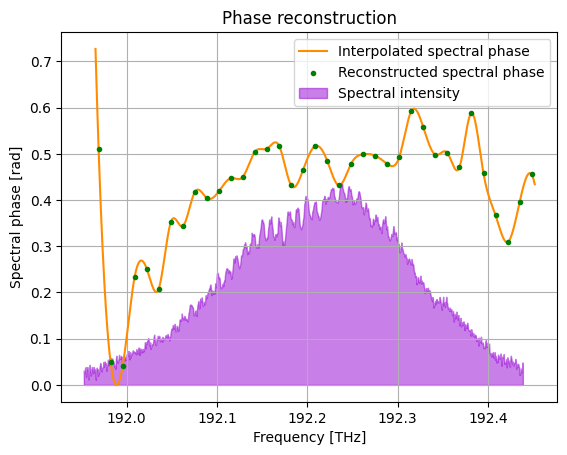
\includegraphics[width=\linewidth]{hg_1}%
}
\vfill
\subcaptionbox*{b) 1st hermite-gauss mode (shear of 11 GHz)}[.7\linewidth]{%
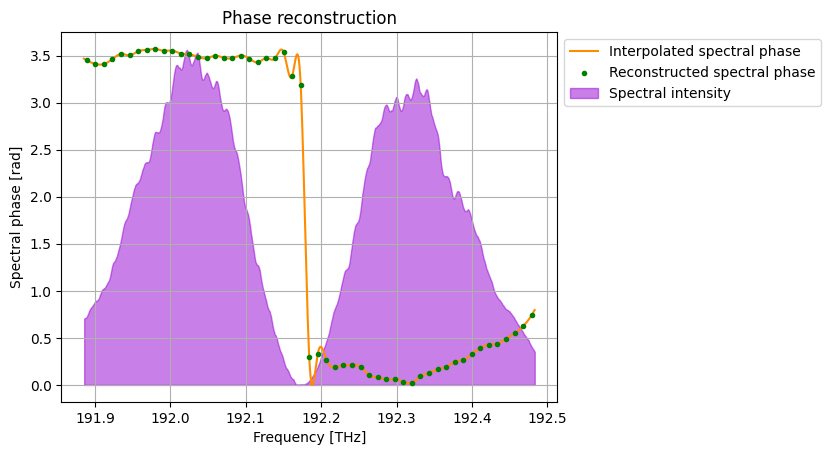
\includegraphics[width=\linewidth]{hg_3}%
}
\vfill
\subcaptionbox*{c) 4st hermite-gauss mode (shear of 11 GHz)}[.7\linewidth]{%
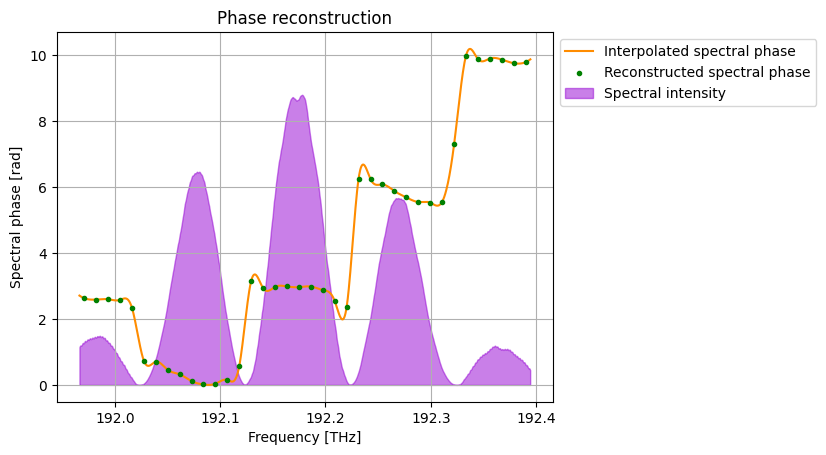
\includegraphics[width=\linewidth]{hg_2}%
}
\label{hermite_1}
\end{figure}

\begin{figure}[H]

\caption{Spectral phase differences of hermite-gauss modes}
\subcaptionbox*{a) 0th hermite-gauss mode}[.52\linewidth]{%
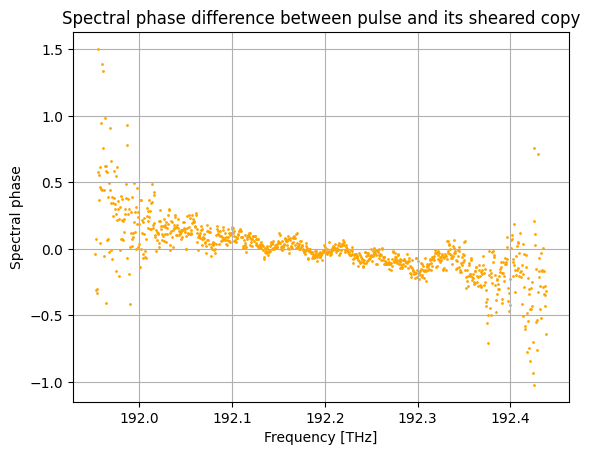
\includegraphics[width=\linewidth]{hg_diff_1}%
}
\vfill
\subcaptionbox*{b) 1st hermite-gauss mode}[.52\linewidth]{%
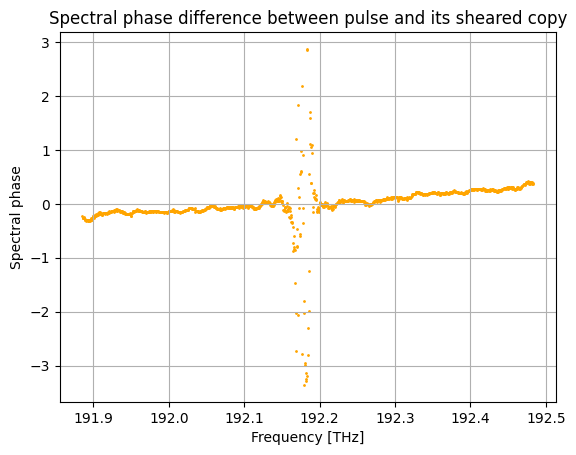
\includegraphics[width=\linewidth]{hg_diff_3}%
}
\vfill
\subcaptionbox*{c) 4st hermite-gauss mode}[.52\linewidth]{%
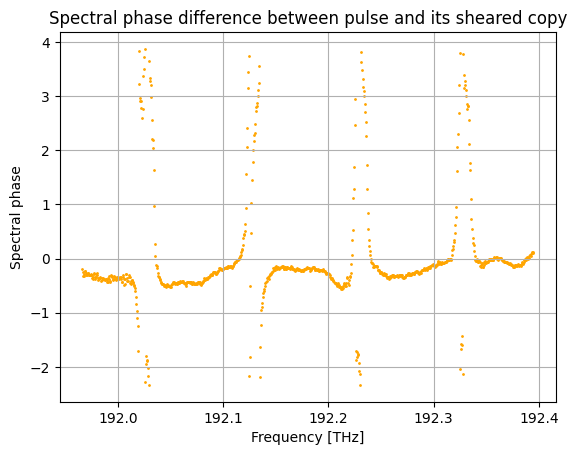
\includegraphics[width=\linewidth]{hg_diff_2}%
}
\label{spd}
\end{figure}

Now, this is pretty interesting! First thing we notice is that each plot contains a slight addition of a linear phase. This is due to to the chirp phase introduced by the fiber that wasn't subtracted yet. Second thing we see is that plot a) definetely contains oscillations with period 65 GHz. In the next measurements I managed to somehow reduce this problem, but still it needs to be solved in a \emph{somehow} clever way, because - for now - 80\% of time needed for conducting a single SPIDER-measurement is associated with positioning the polarization controller in a right position in order to compensate for the wrong alignment of the fiber and the modulator.

The third thing is that the phase in plots b) and c) is definetely \textbf{not} what we expected. What we expect in the case of the first hermite-gauss mode is shown in the fig. \ref{expect}. (Note, that to obtain the below plot, all the measurements were simulated and the entire SPIDER algorithm was employed.)

\begin{figure}[H]
\caption{Simulated spectral phase difference of the 1st hermite-gauss mode}
\centering
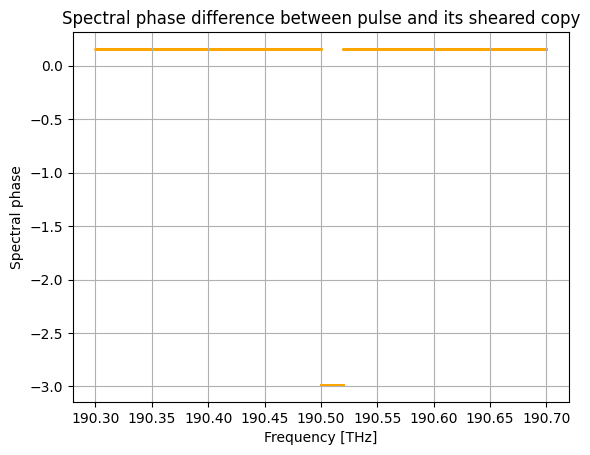
\includegraphics[scale = 0.5]{expect}
\label{expect}
\end{figure}

Let's interprete the above plot. The global phase does not matter, therefore firstly for a long time we have zero. Next, we have a rapid jump by $-\pi$, which is constant for a segment of 20 GHz, which is the value of the shear. This means, that when we \emph{integrate} the spectral phase difference, the value of $-\pi$ will be sampled \textbf{exactly} once corresponding to a single $\pi$-jump of the spectral phase.

However, the plot \ref{spd} b) looks completely differently: instead for a rectangular jump of the spectral phase difference, we have there a noisy peak pointing both up and down! What's more, the support of that peak is around 30 GHz, while the value of shear utilized in experiment was 11 GHz! This means that the fact that the reconstructed spectral phase on the plot \ref{hermite_1} is highly constisted with the model is a matter of a pure luck. If the spectral phase difference had been sampled with the step of 11 GHz, but starting with a different frequency, we could, as well, have a rapid jump of 1 or 2 and not almost excatly $\pi$.

The reason for the noise present in \ref{spd} b) might be the low intensity. This hipothesis is supported by the fact that for the case of 4th hermite-gauss mode, where the low-intensity segements are much shorter, the level of the noise is also lower.

It can be also understood that the peaks are not rectangular, but rather sharp - this might be caused by some diffraction effects or... something like that. However, I have no clue, why the peaks are pointing both up and down.\\
\\

Well, I did hope that I can eliminate the above described problems with an increase of resolution. Luckily, at the same time, I discovered that OSA has a truly beautiful button called \emph{Sensitivity}. I decided to press it.

Having the highest sensitivity of OSA turned on, I managed to perform measurements with shear equal to as little as 2.7 GHz. The result of measurement is shown in fig. \ref{sensitive}

\begin{figure}[H]

\caption{OSA with highest sensitivity - 1st hermite-gauss mode}
\subcaptionbox*{ }[.42\linewidth]{%
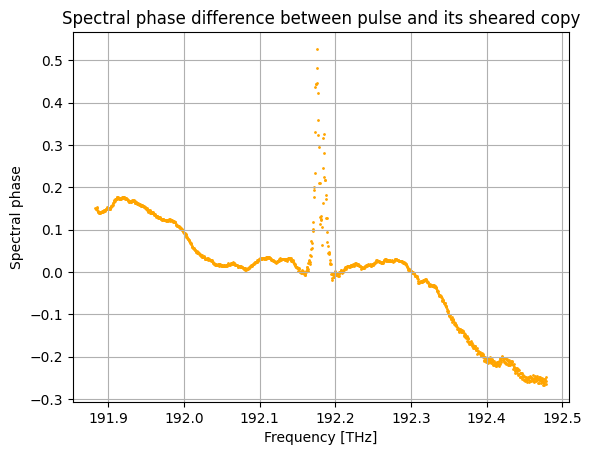
\includegraphics[width=\linewidth]{osa_high_diff}%
}
\hfill
\subcaptionbox*{ }[.58\linewidth]{%
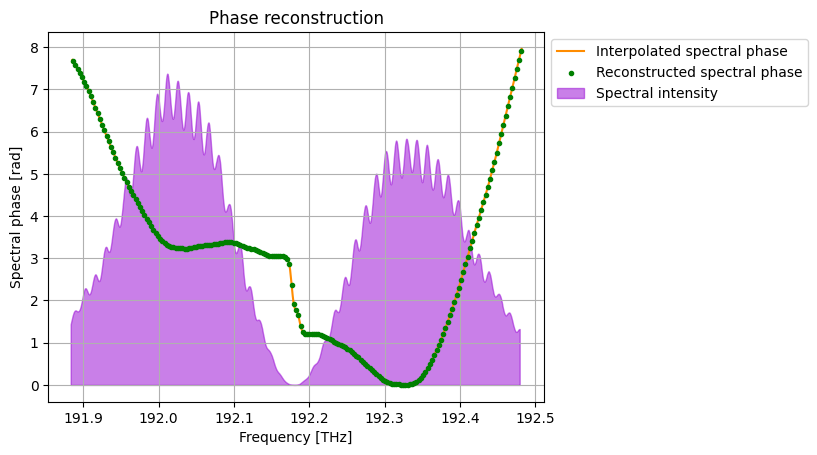
\includegraphics[width=\linewidth]{osa_high_phase}%
}
\label{sensitive}
\end{figure}

The spectral phase difference still contains unsubtracted fiber chirp (hence the linear phase), but overall the level of noise seems to be reduced and the central peak is pointing up only. However, I can not explain, why the spectral phase is \emph{exploding} on the left and right side of the second plot. What is probably the most important is that the width of the central peak (its support or FWHM) is the same as before, although the shear was decreased four times. I conclude that when it comes to increasing the resolution \textbf{the shear is a bottleneck no longer}. What is the reason responsible for smoothening the spectral phase difference? I do not know. But maybe the utilization of the APEX spectrometer can help us to obtain some better results.

\pagebreak
\section{Increasing resolution with APEX}

The resolution of APEX is incredible. Paradoxically this makes quite a problem, because in the optical spectrum measured by APEX all the frequency modes (frequencies supported by the laser cavity) are clearly separated and the spectrum becomes \emph{discrete}. The shape emerging from all the frequency modes combined is called the \emph{optical comb}. Before any other post-processing of measured spectra, one needs to remove this comb. This is done in few steps that are visualized on fig. \ref{decombing}. Note, that only a 0.05 nm long segment of in general 8 nm long spectra are shown on the plots.

\begin{figure}[H]

\caption{Removing optical comb from APEX-measured spectrum}
\subcaptionbox*{a)}[.48\linewidth]{%
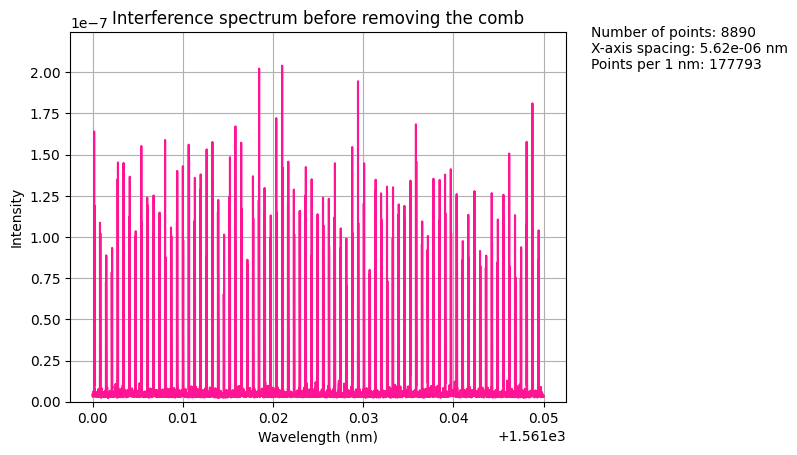
\includegraphics[width=\linewidth]{comb_1}%
}
\hfill
\subcaptionbox*{b)}[.48\linewidth]{%
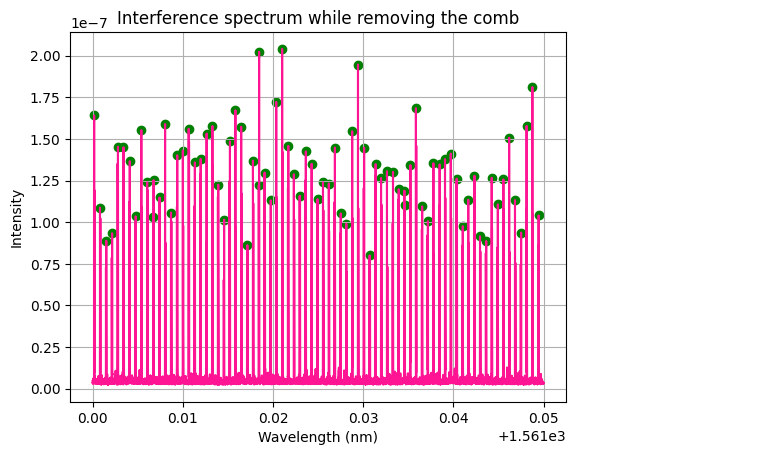
\includegraphics[width=\linewidth]{comb_2}%
}
\vfill
\subcaptionbox*{c)}[.48\linewidth]{%
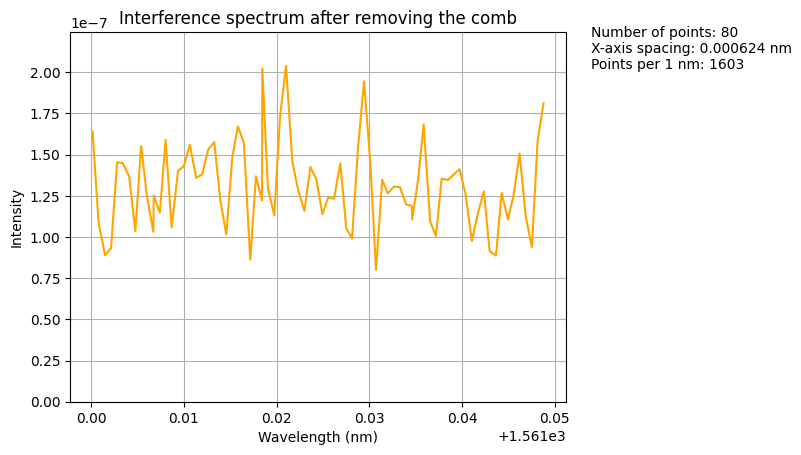
\includegraphics[width=\linewidth]{comb_3}%
}
\hfill
\subcaptionbox*{d)}[.48\linewidth]{%
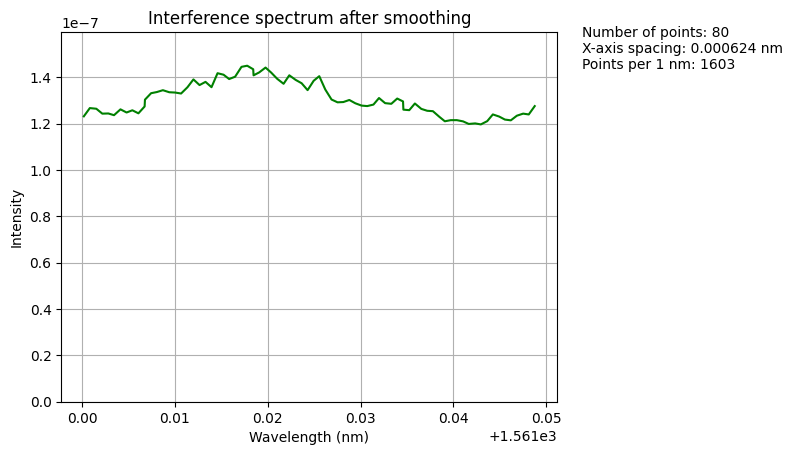
\includegraphics[width=\linewidth]{comb_4}%
}
\label{decombing}
\end{figure}

Despite having very good resolution, the APEX is very noisy (the power of beam guided to APEX was less that 1 $\mu$W at the end), which can be easily noticed in plot c). Therefore also the smoothing, as performed in plot d), was necessary. While removing the comb the number of points constituing the spectrum was decreased more than 110 times. Having this done, I performed the regular SPIDER procedure obtaining the results shown in fig. \ref{apex}. My shear measurements were flawed, therefore I assumed it to be equal to 10 GHz.

\begin{figure}[H]

\caption{Spectral phase measured with APEX}
\subcaptionbox*{a)}[.42\linewidth]{%
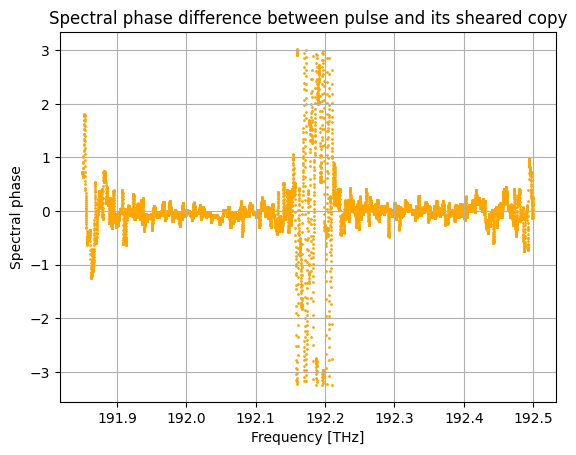
\includegraphics[width=\linewidth]{apex}%
}
\hfill
\subcaptionbox*{b)}[.58\linewidth]{%
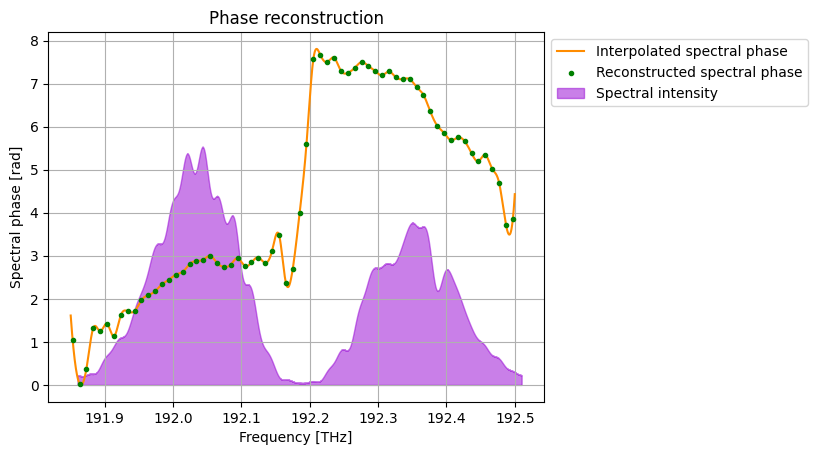
\includegraphics[width=\linewidth]{apex_2}%
}

\label{apex}
\end{figure}

Well... the results are neither great nor terrible. The level of noise is very high, but the reconstructed spectral phase matches \emph{qualitatively} the target. We see again that the amount of subtracted quadratic phase is significantly exaggerated. In the middle of a) plot we have a complete chaos, caused probably by low intensity profile. \textbf{A complete chaos of similar width as the spectral phase difference peaks measured with OSA}, which might suggest that not all the fault is APEX's. Two conclusion come to mind: increase the power of the beam and inspect the phase reconstruction, when the phase jump is in the area of higher intensity. The first thing can be achieved with connecting the erbium doped fiber amplifier (EDFA) to the setup in order not to destroy the pulse shaper by making to much power pass through it. Commenting the second conclusion I could risk the hipothesis that low intensity might be also the reason, why the central peak of the spectral phase difference in previous measuremnts wasn't rectangular. The spectral modes aren't monochromatic and surely some diffraction happens in specrometers or even in fibers. Therefore it is possible that the power can \emph{leak} between very close frequencies, particularly when one of them is much smaller than the second. This can result in local averaging and the \emph{peaky} shape of the peaks. In favour of this hipothesis speaks the constant width of central peak, which seem not to depend neither on the value of the shear nor the type of spectrometer.

\pagebreak

\section{Next steps}

Currently, the main bottleneck in the challenge of increasing the resolution of SPIDER is the wide ($\sim$30 GHz of support, $\sim$10 GHz of FWHM) spectral phase difference peak, where only a narrow, rectangular response should be observed. The width of this peak does not depend neither on value of the shear nor on the type of spectrometer (OSA, APEX). This effect is best to be seen in fig. \ref{spd_problem}. The measurement, whose full outcome was also presented in fig. \ref{sensitive}, was used.

\begin{figure}[H]
\caption{Problem with spectral phase difference}
\centering
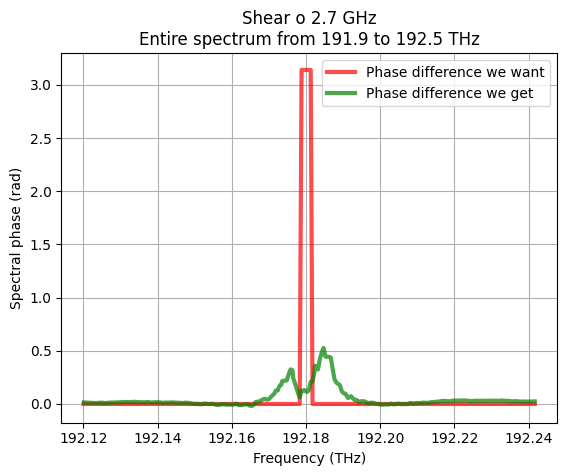
\includegraphics[scale = 0.7]{spd_problem}
\label{spd_problem}
\end{figure}

Emm... this measurement was performed with OSA, but the M-shaped outcome, when a \emph{monochromatic} response is expected, disturbingly resembles the (fundamental) behaviour of APEX... I have a feeling that my model is completely wrong.

To be honest, it is a pure coincidence that I noticed this M-shape, which is not visible in normal scale (look at the left plot in fig. \ref{sensitive}). I just wanted to plot a zoomed version of my most stable measurement, because the shear used here was very small...

I am quite shocked. I though that the shape of the central peak should be associated mainly with noise, while this M-shape looks like something that can be very nicely modelled (and maybe removed in post-processing).

\pagebreak

Nonetheless, I have also other solutions that may reduce noise, oscillations and time needed for performing a spectral phase measurement. Here they come:

\begin{enumerate}
\item \textbf{Align fibers connected EOPM}\\
This is a matter of primary importance, discussed by me already in my bachelor thesis. The axes of optical fiber connected to EOPM are rotated by a few degrees in respect to axes of lithium niobate crystal, which results in oscillations in spectrum with the period of 65 GHz. Currently, I am compensating for this effect using the polarization controller, which is an inaccurate, time-consuming and annoying procedure (1st SPIDER measurement takes around 30 min, the next, with polarization controller already fixed, less than 4).

\item \textbf{Measure dispersion parameter in a separate measurement}\\
The exact (at least to 1 decimal place) value of the dispersion parameter is needed for estimating the amount of quadratic chirp phase introduced by the delaying fiber. Measuring this quantity is crucial, because without it is is impossible to find the values of the initial chirp and the additional chirp in EOPM and thus to estimate value of quadratic phase needed to be subtracted in post-processing.

\item \textbf{Simulate what happens when the current steering the modulator is not entirely linear}\\
Probably it is sufficient to just consider the quadratic and cubic correction. Inspect behaviour of the phase and check, how important it is to for the current to be fully linear.

\item \textbf{Write the program checking in real time, if the applied shear is homogenous}\\
Using code given to me by Ali Golestani I am able to connect a Python program to OSA in real time and inspect the linearity (or rather the homogeneity) of the spectral shift. This can be achieved by minimizing the difference between the shifts of left and the right spectrum's slopes or by minimizng MSE between original spectrum and \emph{numerically de-shifted} sheared spectrum. Of course, the \emph{shape} of the shear is controlled indirectly by the delay line.

\item \textbf{Find out what might be the reason for additional quadratic phase, as described in Section \emph{Stability}}\\
As discussed before, although the reconstructed spectral phase is almost perfectly quadratic, the coefficient before the parabola is scaled. The scaling is constant within a single serie of measurements. Proposed explanation of this phenomenon include initial chirp occuring already in the laser cavity, chirping due to the nonlinearity of current, chirping due to non-zero mean intensity of current passing through EOPM, optical rectification in  the modulator, a systematic error in shear measurement and modulation of non-modulated polarization in the modulator. I must propose a model that predicts quantitatively the additional quadratic phase.

\item \textbf{Measure a spectrum with a rapid spectral phase jump in the area of high intensity}\\
One of possible explanation for unexpected behaviour of the spectral phase difference is assuming that it connected with the rapid spectral phase jump in the are of almost zero intensity. Especially in the case of APEX, changing the place of phase jump, may significantly improve the results.

\item \textbf{Connect an EDFA to the setup with APEX}\\
APEX is noisy when the input signal is low. And the input signal in my experiments was terribly low, as only about 1/4000 of initial beam manage to propagate through entire setup (greatest losses in the modulator and in the pulse shaper). A solution, which should not damage the pulse shaper, is to connect an EDFA after the pulse shaper and before the APEX.

\item \textbf{Consider switching from the photodiode to RF generator}\\
The RF generator may provide a better control of the current's linearity and allow us to measure greater spectral phases. Currently, when the chirp phase is introduced by more than 150 m of fiber, the optical pulse gets so long that it becomes impossible to make it overlap with a linear slope of the current. This problem may by solved with an application of the RF generator.
\end{enumerate}
\end{document}